\subsection{Jet reconstruction}
\label{sec:4.1}

Jets are defined in two way:  Monte Carlo (MC) simulated jets at particle level and detector level jets with the information from the ID and calorimeters. The production and hadronisation processes of jets are illustrated in Figure~\ref{Fig.jet}.

\begin{figure}[htb] 
	\centering  
	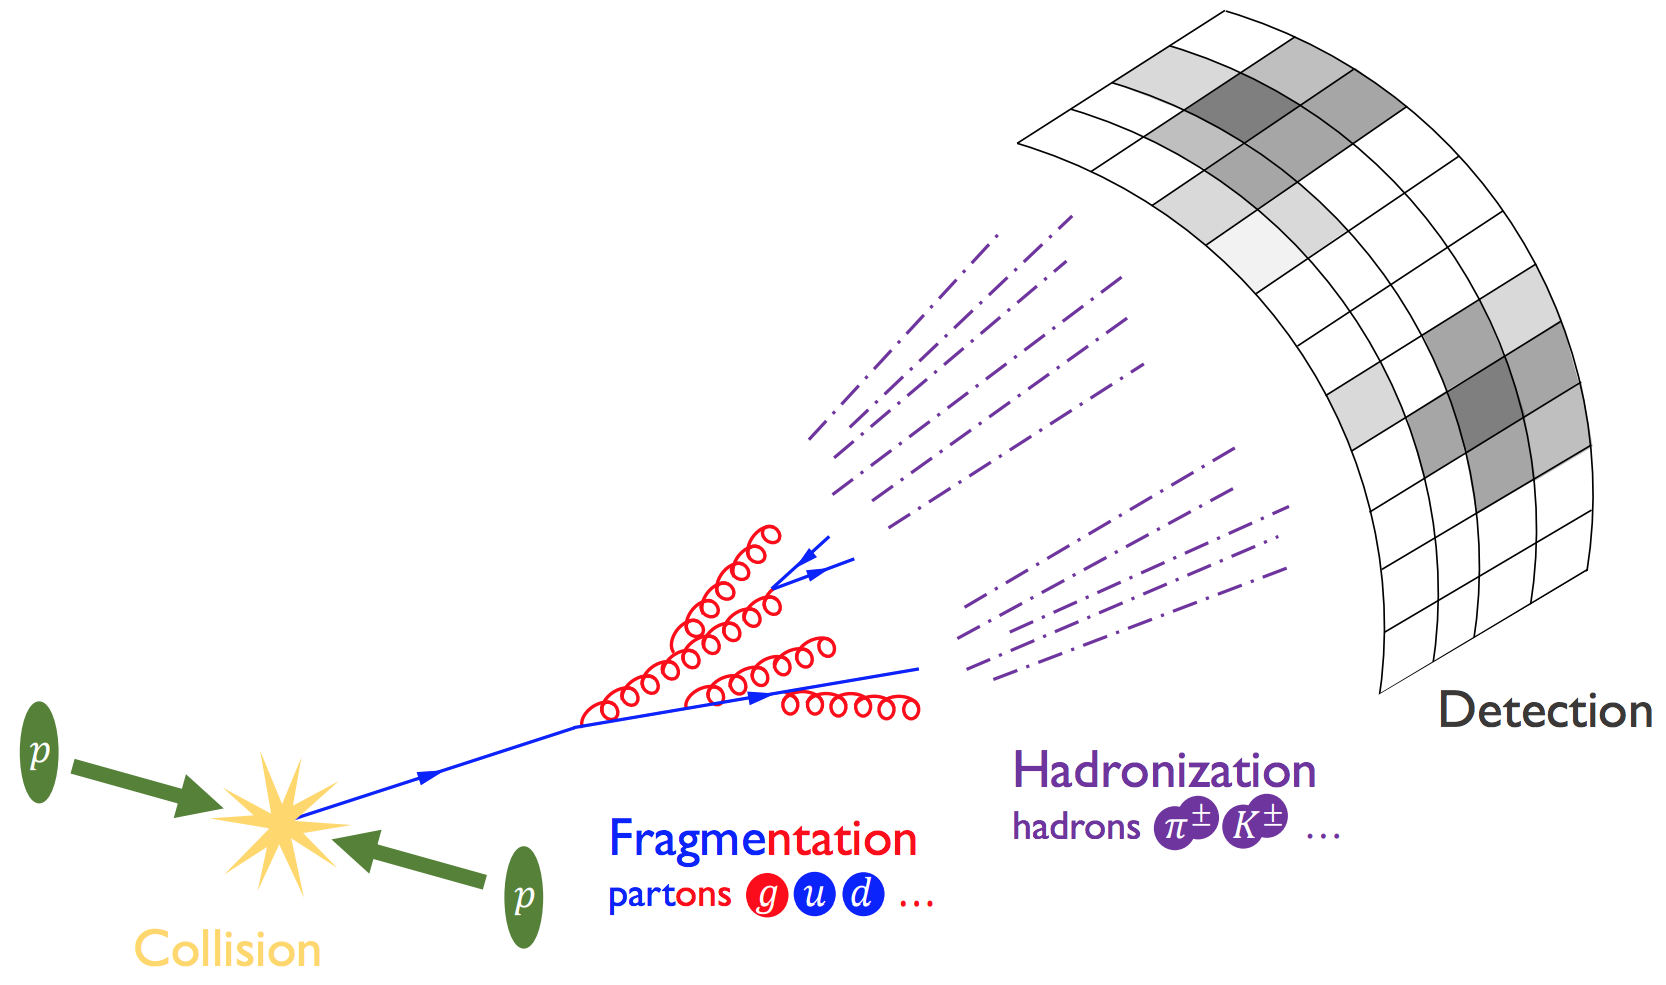
\includegraphics[width=15cm]{./fig/jet.jpg}	\caption{illustration of jets produced by pp collision and hadronised before seen by the detector.}
	\label{Fig.jet}
\end{figure}

Jets from the MC simulation are defined as truth-particle jets which have lifetimes longer than 10 ps as stable particles. Truth-particles indicate the ideal measurement from a detector under perfect-condition and high resolution without defects or the effects from pile-up (background interactions per bunch-crossing in the LHC). Whereas track jets are constructed with the use of charged information in the ID, and calorimeter jets with the use of energy information in the calorimeters.

There are several types of jets aim for different analysis depended on the constituents and algorithm used for reconstructing the jets. ATLAS previously used topo-cluster jets, which is a group of topological related cells in calorimeter with significantly high energy deposits. A pile-up suppressed algorithm is applied to select certain cells with low noise. Cell above certain signal-to-noise (S/N) threshold (usually by four times its standard deviation) are used to seed the algorithm. By neighbouring the seed a topo-cluster is defined. In the hard-scatter process, jets of interest are expected to produced from the primary interaction point (known as vertex). The primary vertex is defined if there are at least two tracks with the highest sum of squared track momentum associated to it.

Jets are constructed from any set of four-vectors. EMTopo jets are the jets that use topo-cluster initially calibrated to electromagnetic (EM) scale in the calorimeters. A local cluster weighting (LCW) scale is also used for calibrating hadronic clusters by applying weights for low hadronic interaction response. Besides, particle flow (PFlow) jets are built by combining the information from both the ID and the calorimeter, where the energy deposited from the calorimeter are removed by the momentum in the ID by a cell-based energy subtraction algorithm. The inputs to the particle flow algorithm are the separate topo-clusters with local energy maxima, respectively. 

A recombination algorithm called anti-$k_t$ algorithm is employed to build the jets with a radius parameter $R$ in rapidity-azimuth $(y-\phi)$ plane around a cluster. The algorithms are defined as follows:

\begin{equation}
d_{i j}=\min \left(k_{\mathrm{t} i}^{2 p}, k_{\mathrm{t} j}^{2 p}\right) \frac{\Delta_{i j}^2}{R^2}
\end{equation}

\begin{equation}
\Delta_{i j}^2=\left(y_i-y_j\right)^2+\left(\phi_i-\phi_j\right)^2
\end{equation}

\begin{equation}
d_{i B}=k_{\mathrm{t} i}^{2 p}
\end{equation}
where the distance $d_{i j}$ between any pair of particles $i$ and $j$ is given by the minimum transverse momenta $k_t$ of the two particles. The geometrical distance $\Delta_{i j}$ represents the separation of a pair of particles in $(y-\phi)$ plane. Radius parameter $R$ indicates the size of the final jets. The distance $d_{i B}$ between any detected particle i and the beam $B$ is also given. Parameter $p$ indicates the relative power of of energy with respect to geometrical scales and is used to distinguish the different types of algorithms.

When $p$ is set to 0,  the Cambridge-Aachen (CA) algorithm is given as the distance $d_{i j}$ and $d_{i B}$ only based on spatial separation and are independent of the transverse momenta. This algorithm is usually used for large-radius jets and jet substructure performance study.

For the $k_t$ algorithm, $p$ is set to 1 so that the distance $d_{i j}$ is dominated by the minimum $k_t$. This algorithm is preferred for clusters that are soft and collinear splits are merged first, resulted in irregular footprint with the most interesting splits.

The  \antikt~algorithm on the other hand set $p$ = -1, leaving the distance $d_{i j} \propto \min \left(\frac{1}{k_{t i}^2}, \frac{1}{k_{t j}^2}\right)$ shorten as the transverse momenta of two particles increase. This is widely used in the LHC for hard clustering as it is less vulnerable to the effects from the pile-up and resulted in circular footprint as shown in Figure~\ref{Fig.kt} for $R = 1.0$.

\begin{figure}[htb] 
	\centering  
	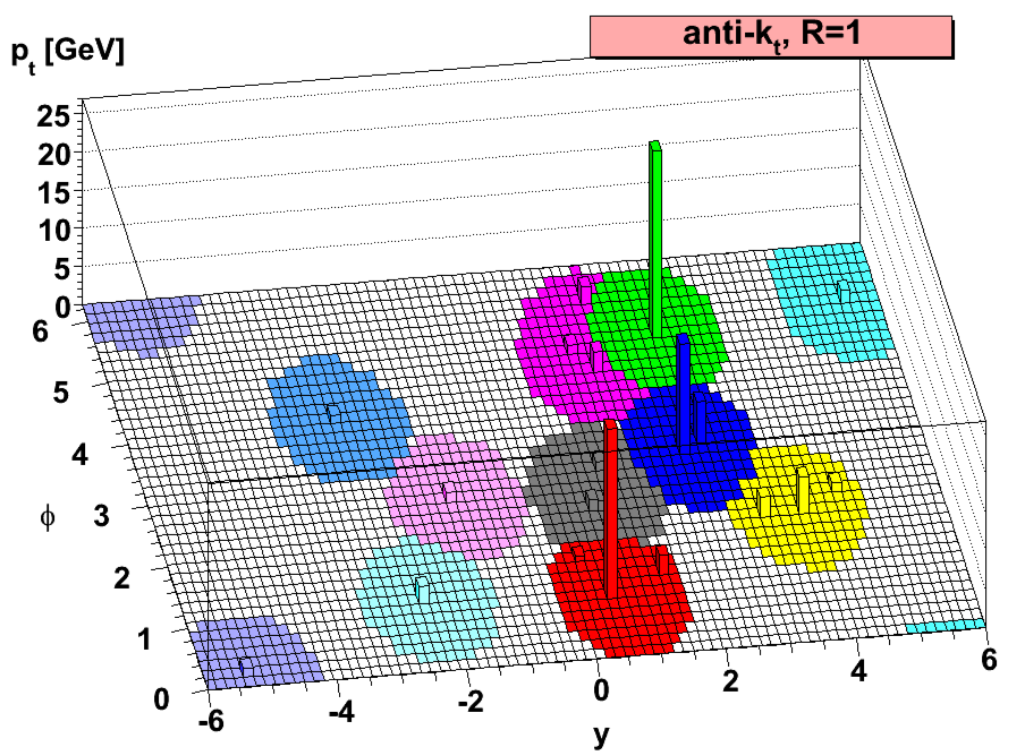
\includegraphics[width=12cm]{./fig/kt.png}	\caption{Plot of parton-level jets clustered using  \antikt~algorithms with radius parameter set to 1.}
	\label{Fig.kt}
\end{figure}

For most of ATLAS analysis, jets with $R = 0.4$ are used for quarks and gluons analysis. Other ones such as $R = 1.0$ are also widely used to study energetic particles like W and Z bosons. $R$ = 0.2, 0.6, 1.2, 1.5 and variable radii are also analysed.

The \antikt~$R = 0.4$ PLow jets are used in the quark/gluon taggers calibration described in this thesis.



\subsection{Jet calibration and cleaning}
\label{sec:4.2}

The motivation of jet calibration is to correct the translation from received signals to initial partons for several detector effects, including energy deposited in dead or beyond areas in the detectors, low response to hadronic reactions, pile-up, radiations that outside jet cone, etc. The calibration process is thus needed to account for the energy of jets to that of MC simulated jets at particle-level.

Calibration is performed to topological clusters at the EM scale where the sum of the energies in all constituent cell are taken, or at the LCW scale where low hadronic response in the ATLAS calorimeters is taken into account. The diagrams~\ref{Fig.calib} shows the calibration scheme for small-$R$ jets.

\begin{figure}[htb] 
	\centering  
	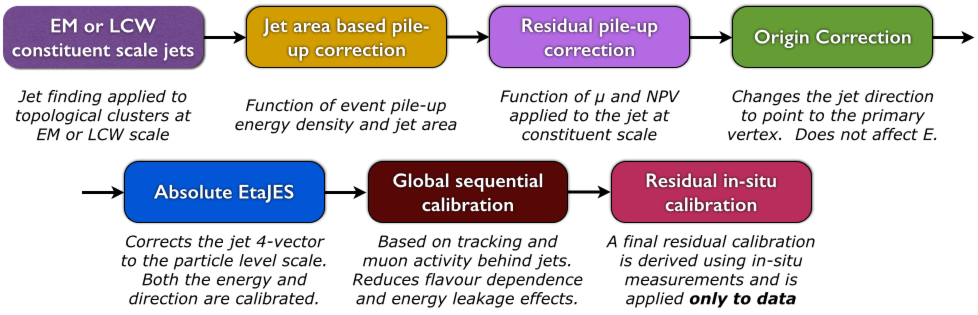
\includegraphics[width=15cm]{./fig/calib.png}	\caption{Overview scheme of jet calibration in the ATLAS.}
	\label{Fig.calib}
\end{figure}

\subsubsection{Pile-up corrections}


In order to eliminate a great amount of energy deposits from pile-up, a jet area-based subtraction of pile-up contribution to the \pt of each jet per event is applied as the start of the calibration chain. 

After all pile-up corrections are applied, the jet \pt~is given by:

\begin{equation}
p_{\mathrm{T}}^{\text {corr }}=p_{\mathrm{T}}^{\text {reco }}-\rho \times A-\alpha \times\left(N_{\mathrm{PV}}-1\right)-\beta \times \mu
\end{equation}
where $p_{\mathrm{T}}^{\text {reco }}$ indicates the reconstructed jet \pt~before any pile-up correction is applied. The jet area $A$ is defined by certain number of ghost tracks associated with a jet after clustering thus can quantify the liability of a jet to pile-up.  The pile-up \pt~density $\rho$ is used to evaluate the contribution from pile-up in the y-$\phi$ plane. To calculate the density $\rho$ of each jet in the distribution $\pt/A$, a $k_t$ algorithm with radius $R$ = 0.4 is employed to reconstruct jet from positive-energy topo-clusters within the range of \abseta < 2. The calculation of $\rho$ performed in such $\eta$ range for pile-up measurement is due to the fact that $\rho$ tend to be zero beyond \abseta~$\approx$ 2 as a result of lower occupancy in coarser segmentation in the forward region. Therefore, pile-up sensitivity in the forward region is not fully described after such correction.  

An additional residual correction is thus applied from the MC simulation to account for the difference between the reconstructed jet \pt~and truth jet \pt~as a function of the number of reconstructed primary vertices in the event $N_{\mathrm{PV}$  and the mean number of interactions per bunch crossing $\mu$, which are sensitive to in-time and out-of-time pile-up, separately. 

Both the initial values of $\alpha$ and $\beta$ coefficients are derived in bins of truth jet \pt~and geometric centre of the detector $|\eta_{det}|$. A logarithmic dependence on truth jet \pt~is observed.


\subsubsection{Jet energy scale and $\eta$ calibration}

Following the pile-up mitigation, the absolute jet energy scale and $\eta$ calibration are introduced to correct the four-momentum of the reconstructed jet to the truth-particle jets, accounting for defecting calorimeter response, energy losses when particles passed through certain materials, boundary effects and biases in the reconstructed jet in different $\eta$ due to the transition between the granularities and technologies changes in calorimeter. 


Since the detector responses differ across the detector $\eta$ range, the reconstructed jets are thus divided into small bins of $\eta_{det}$ and the energy of the truth jet $E^{truth}$ as the response distribution for fixed $E^{truth}$ is Gaussian. The average jet energy response $\mathcal{R}$ is defined as $E^{\text {reco }} / E^{\text {true }}$ using  the mean of a Gaussian fit in $\eta_{det}$ and $E^{truth}$ bins, and is further parameterized as a function of $E^{reco}$. Such response for PFlow jets is higher than that for EMtopo jet at low energies as the tracking information is considered. 


Besides Jet energy scale (JES) correction, the bias from the $\eta$ of the reconstructed jet to that of the truth jet is taken into account. The bias is defined as a significant deviation from zero in the signed difference between the reconstructed jet $\eta^{reco}$ and truth jet $\eta^{truth}$, separately. Then a second correction is applied as such difference is parameterized as a function of $\eta_{det}$ and $E^{truth}$.

 The calibration is derived as a function of energy and $\eta$ from the MC samples which do not have the effects from pile-up, and only correct the jet \pt~and $\eta$ instead of full four-momentum. The EMtopo and PFlow jets after full JES and $\eta$ calibration are regarded as EM+JES scale and PFlow+JES scale, respectively. Small non-closures beyond $|\eta_{det}|$ $\approx$ 3.2 in the calibration are seen due to approximate treatment of hadronic showers in the forward region, lead to an additional systematic uncertainty.


\subsubsection{Global sequential calibration}

The global sequential calibration (GSC), based the global jet observables such as the the fraction of jet energy measured in the different layer of hadronic and the EM calorimeters, the tracking information associated with the jets, and the number of muon track segment. For each observable, a series of multiplicative corrections are applied on the four-momentum as a function of $\pt^{truth}$ and $|\eta_{det}|$.  Considered any observable $x$, the correction is derived from the inverted jet response $\mathcal{R}$:

\begin{equation}
C(x)=\frac{\mathcal{R}^{-1}}{\left\langle\mathcal{R}^{-1}(x)\right\rangle}
\end{equation}
where $\left\langle\mathcal{R}\right\rangle$ is the average jet response. 

As a result, the fluctuations in the jet particle composition are reduced and the jet resolution can be improved without changing the average jet energy response which depends on the flavour and the energy distribution of the constituent particles. The shape of a jet varies between quark- and gluon-initiated jets as hadrons are often included in a quark-initiated jet with higher fraction of the jet \pt~with higher calorimeter response.

After applied GSC for PFlow jet, the average jet \pt~ response on each observable is reduced to lower than 2\% with small deviations from correlations between observables.


The fractional jet resolution $\sigma_{\mathcal{R}} / \mathcal{R}$ is derived from the jet resolution $\sigma_{\mathcal{R}}$, which is defined by the standard deviation of a Gaussian fit to the distributionof  jet \pt~response. This fractional jet resolution is used to determine the size of the fluctuations in the jet energy reconstruction.



\subsubsection{Residual $in~situ$ calibration}

The final step of the jet calibration is performed only in data to account for the differences of jet response measurement in data and the MC, the derived ratio of it is used as a correction in data.
The differences are introduced by the inadequate nature of the detector materials and the imperfect simulation of the real physics processes. Such differences can be quantified by weighting the \pt~ of a jet to other reference objects that well-measured. The correction factor  can be denoted as follows:
\begin{equation}
c=\frac{\mathcal{R}_{\text {in situ }}^{\text {data }}}{\mathcal{R}_{\text {in situ }}^{\mathrm{MC}}}
\end{equation}
the response $\mathcal{R}_{\text {in situ}}$ represents the average ratio of the jet \pt~ to the reference object \pt~ in bins of reference object \pt, where the average value is founded from peak value of a Gaussian fit to the distribution. The double ratio is robust to secondary effects thus more reliable in term of the measurement of jet energy.

Three stages are carried out in such $in~situ$ calibration. First, $\eta$-intercalibration is performed on the energy scale of forward jets (0.8 $\leq |\eta_{det}|$ < 4.5) to match the central jets ($|\eta_{det}|$ < 0.8) using the jet \pt~in dijet events. Then $Z$+jet and $\gamma$+jet analyses balance the measurement of \pt~response of a well-calibrated $Z$ boson or photon. Finally, a multijet balance (MJB) analysis is employed to calibrate low-\pt~jets to a very high-\pt~jet. Both MJB and $Z/\gamma$+jet analyses are used only for jets in the central region (\abseta < 1.2). All three $in~situ$ calibrations are done sequentially so that the systematic uncertainties can be propagated from each to the next. The systematic uncertainties in each calibration process come from three sources: the MC modelling of physics processes, the uncertainties in the measurement and from topology obtained by different event selections.




